\chapter{Systementwurf}\label{chp:systementwurf}
%Auf der Basis des Pflichtenhefts werden aus softwaretechnischer Sicht die Anforderungen an das System spezifiziert. Hierzu gehört minimal eine Beschreibung auf höherem Niveau (Modulebene), eine auf mittlerem Niveau (Struktogramme, Pseudocode oder Spezifikation von Prozeduren (Funktionen) sowie die Beschreibung der für das System essentiellen Datenstrukturen (z.B. als Datenlexikon). Typische Beschreibungen sind die Modulhierarchie (oder Modulgraph), eine Spezifikation aller Module mit ihren Schnittstellen (inklusive Zweck, Ein-/Ausgabe), sowie eine Spezifikation aller in den Modulschnittstellen liegenden Prozeduren und Funktionen.
%Bestandteil des Entwurfs sollten nicht nur die jeweiligen Ergebnisse, sondern auch die Beschreibung des Entwicklungsweges (inklusive verworfener Lösungen) sein.

\section{Klasse Window}
\paragraph{}
Die Klasse \textit{Window} baut die Benutzeroberfläche auf und speichert die Eingabe des Benutzers in Variablen. Diese Werte werden dann an die Klasse \textit{Interpreter} weiter gegeben. In der Benutzeroberfläche werden die Eigenschaften für jeden Testvorgang eingestellt.


\subsection{Design}
\begin{figure}[h]
  \begin{center}
    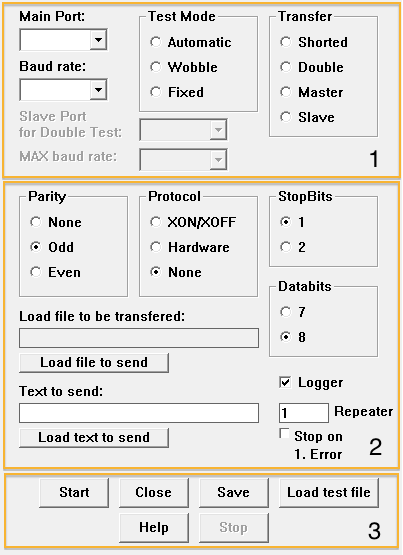
\includegraphics[scale=0.6]{gui.png}
  		  \caption{Design der Benutzeroberfläche}
     \label{GUI_Bild}
  \end{center}
\end{figure}


Die Benutzeroberfläche ist in drei Abschnitte geteilt. Die verschiedene Abschnitte sind in der Abbildung \ref{GUI_Bild} zu erkennen. Genaueres zu alle Parametern wird in Kapitel \ref{chp:bedienungsanleitung} und  \ref{chp:fachlichesumfeld} erläutert. Der erste Abschnitt von Einstellungen hantieren die Testeinstellungen. Diese Einstellung sind:
\begin{itemize}
\item Main Port: welcher COM Port soll getestet werden.
\item Baud rate: beschreibt mit welcher Baudrate der ausgewählte Port getestet werden soll.
\item Test Mode: definiert welcher Testvorgang der Benutzer haben möchte.
\item Transfer: legt fest, wie die Kommunikation dieses Ports stattfinden wird.
\end{itemize}


Die zwei ausgegrauten Einstellungen ("`Slave Port for Double Test"' und "`MAX baud rate"') sind abhängig vom Testmodus und Transfermodus.\\

Der zweite Abschnitt sind die Übertragungsparameter und drei weitere Testeinstellungen. Diese Parameter sind:

\begin{itemize}
\item Parity: Paritätsüberprüfung
\item Protocol: Übertragungsprotokoll
\item Stopbits: Anzahl der Stopbits
\item Databits: Anzahl der Datenbits
\item Logger: definiert ob eine Log-Datei erstellt werden soll
\item Repeater: Anzahl der Testwiederholungen
\item Stop on 1. Error: bestimmt ob bei der ersten Fehlererkennung angehalten werden soll
\item Load file to be transfered: Übertragungsdatei der übertragen wird
\item Text to send: Übertragungstext der gesendet wird\\
\end{itemize}

Die letzte Reihe von Elementen in der Benutzeroberfläche sind die Schaltflächen. Diese führen die jeweiligen Vorgänge aus.

\begin{itemize}
\item Start: startet einen Test
\item Close: schließt das Test Tool
\item Save: speichert in eine Testdatei mit den Einstellungen
\item Load test file: lädt eine Datei die im Test übertragen wird
\item Help: zeigt ein Fenster mit Erklärungen zum Test Tool
\item Stop: stoppt der laufende Test\\
\end{itemize}

Beim Drücken des Start-, Save- oder "`Load test file"' Schaltfläche werden die Testeinstellungen an die Klasse \textit{Interpreter} weitergegeben und dort werden diese verarbeitet.


\subsection{Aufbau}
\paragraph{}
Die Klasse \textit{Window} erbt von der \textit{Template class} in der Headerdatei \textit{BaseWindow}. Die Headerdatei beinhaltet die Definition des Templates. Im Template, wird die für die Nachrichtenschleife nötige, statische Fensterprozedur deklariert. Hier wird nur nach die Nachricht \textit{WN\_NCCREATE} abgefragt, wie bereits im Kapitel \ref{C++GUILoesung} erwähnt wurde. Wenn die Nachricht empfangen worden ist, werden die weitere Nachrichten an das Handle des Fensterobjekt weitergeleitet. In dem Template wird außerdem auch eine Fensterklasse deklariert, registriert und danach erzeugt. Somit werden alle Nachrichten eines Fensterobjektes immer zuerst an die statische Fensterprozedur gesendet, diese leitet durch einen Zeiger und ein Handle die Nachricht an das korrekte Fenster weiter. Um genauer die Funktionalität des Templates zu verstehen, siehe bitte Anhang \ref{TemplateClass}.

\subsection{Aufgaben}
\paragraph{}
Die Klasse hinter der Benutzeroberfläche besteht aus zwei Teilen. Der erste Teil bearbeitet die Eingabe des Benutzer und den Aufbau der Oberfläche, der zweite Teil die Weitererarbeitung der Daten.\\

Der erste Teil besteht aus der Methode \textit{HandleMessage}, diese Methode ist die Fensterprozedur. Als erstes werden die Elemente, mit der Ankunft der Nachricht \textit{WM\_CREATE}, des Fensters aufgebaut. Danach wird auf die Nachricht \textit{WM\_COMMAND} gewartet und jeweils reagiert. Wird zum Beispiel die Start Schaltfläche gedrückt, bekommt die \textit{HandleMessage} Methode die \textit{WM\_COMMAND} Nachricht mit dem Parameter \textit{ID\_BT\_START}, dass ist die Identifikationsnummer im Programm für die Startschaltfläche.\\

\begin{lstlisting}	 
    case WM_CREATE:
        {
            //Erzeuge alle GUI Elemente
            
            //example: Start button
            _hwnd_Start = CreateWindowA("button", "Start",
				WS_CHILD | WS_VISIBLE,
				POS_X + 20, POS_Y2 + 290, 70, 30, m_hwnd, (HMENU)ID_BT_START,
				NULL, NULL);
        }
        break;
\end{lstlisting}

Wenn die Startschaltfläche gedrückt worden ist, fängt der zweite Teil der Klasse an. Der zweite Teil besteht aus der Weiterverarbeitung der Eingaben. Im Fall der Startschaltfläche, wird als erstes ein neuer Thread erzeugt. So kann die Benutzeroberfläche immer noch Nachrichten verarbeiten, während im Hintergrund das Programm die Datenverarbeitung beginnt. Der gleiche Vorgang geschieht, wenn die \textit{Load test file} Schaltfläche gedrückt wird.\\

Im Fall von der Startschaltfläche, ruft der Thread die Methode \textit{sendTestSettings} auf, die die Eingaben weiter an ein Interpreter-Objekt gibt. Dies geschieht in dem ein Objekt der Klasse \textit{Interpreter} erzeugt wird und dessen Eigenschaften gesetzt werden.

\begin{lstlisting}	 
	case WM_COMMAND:
	{
		//Reagiere auf Klicks der Schaltfäche
		//Beispiel: Startschaltfläche
		case ID_BT_START:

			//augrauen der Elemente während ein Test
			viewAllElements(FALSE);

			//erzeuge ein neuen Thread
			_t1 = thread(&Window::sendTestSettings, this);

			//abtrennen des Threads für den Test, während der Mainthread
			//auf Stopp wartet oder die Beendigung des Tests
			_t1.detach();
	}
    break;
\end{lstlisting}




%****************************************************************************************
\newpage
%****************************************************************************************

\section{Klasse Interpreter}
\paragraph{}
Die Klasse \textit{Interpreter} trennt die Benutzeroberfläche von der Fachlogik des Programms. Die Benutzeroberfläche kann den Interpreter aufrufen und hat Zugriff auf die \textit{public} Methoden der Klasse. Der Interpreter kann nicht auf Elemente oder Methoden der Klasse \textit{Window} zugreifen. Durch diese Trennung kann der Benutzer nie "`unkontrolliert"' auf die Fachlogik zugreifen, nur über die Möglichkeiten die der Programmierer ihn anbietet.\\

\subsection{Aufgaben}
\paragraph{}
Eine Aufgabe des Interpreters ist die Überprüfung der Eingaben des Benutzers, bevor die Tests beginnen. Durch so genannte "`setter"'-Methoden werden die Eingabeparameter der GUI in lokalen Variablen gespeichert.\\


\begin{lstlisting}	 
void Interpreter::setTransfer(int iTransfer)
{
	this->_iTransfer = iTransfer;
}
\end{lstlisting}

Danach werden die lokalen Variablen auf Fehleingaben geprüft. Sind Fehler erkannt worden, werden diese dem Benutzer bekannt gegeben und alle Parameter in der Klasse werden auf ein Standardwert zurückgesetzt. Sind keine Fehleingaben erkannt worden, werden die Werte der Variablen in einer Datenstruktur gespeichert. Mehr zu dieser Struktur wird im Kapitel ~\ref{TestStruct} behandelt. Im folgenden Quellcode wird eine Fehlerüberprüfung dargestellt, hierbei handelt es sich um den Übertragungsmodis, der abgefragt wird.

\begin{lstlisting}	 
if (_iTransfer == DEFAULT_VALUE)
{
	MessageBoxA(NULL,"Bitte wählen Sie ein Transfermodus aus",
							WINDOW_TITLE, MB_OK | MB_ICONERROR);
	setDefaultValues();
}
else
{
	//speichern des Transfermodus
	_testManager->testStruct.iTransfer = _iTransfer;
}
\end{lstlisting}

Die Werte in den Variablen müssen überprüft werden, um Fehler zu vermeiden. Da die Werte nicht nur aus Einstellungen in der Benutzeroberfläche stammen, sondern auch aus einer Testkonfigurationsdatei, können falsche Eingabe vorhanden sein. Zusätzlich zur Überprüfung der Eingabeparameter und setzen der lokalen Variablen, gibt die Klasse \textit{Interpreter} die Testeinstellungen an die anderen Klassen weiter. Hier trennt sich das Programm in zwei Pfade. Der erste Pfad gibt die Datenstruktur an die Klasse \textit{TestManager} weiter. Der zweite Pfad speichert oder liest eine Testkonfigurationsdatei aus. Im Fall, dass eine Testkonfigurationsdatei gelesen werden soll, wird als erstes die Klasse \textit{IniFileHandler} aufgerufen und danach die Klasse \textit{TestManager}, um ein Test mit den gelesenen Einstellungen zu starten. Sollen die Eingabeparameter der Benutzeroberfläche in einer Testkonfigurationsdatei gespeichert werden, werden die überprüften Eingabeparameter in einer vom Benutzer angegebene Datei gespeichert. Dafür wird auch die Klasse \textit{IniFileHandler} aufgerufen.\\

Da die Klasse \textit{Interpreter} die Schnittstelle für die Kommunikation zwischen Fachlogik und der Benutzeroberfläche ist, wird auch durch diese Klasse die Meldung gegeben, ein Test anzuhalten. Durch das Klicken der Schaltfläche "`Stop"' in der Benutzeroberfläche wird eine boolesche Variable weiter an die Testlogik gegeben. Diese Variable wird vor jeder Testschleife abgefragt, ist sie gesetzt, dann wird der Test angehalten.\\

Die Klasse hat ein Objekt der Klasse \textit{Com}, um in der Benutzeroberfläche die im System zur Verfügung stehenden COM Ports aufzulisten. Durch die Trennung der GUI von der Fachlogik, darf die \textit{Window} Klasse kein Objekt der Klasse \textit{Com} haben.\\



%****************************************************************************************
\newpage
%****************************************************************************************

\section{Struktur TestStruct}\label{TestStruct}
\paragraph{}
Eine \textit{struct} oder Struktur dient dazu, mehrere logische zusammenhängende Variablen verschiedener Datentypen zusammenzufassen. In \textit{C} beinhalten Strukturen nur Variablen, in \textit{C++} wurden die Strukturen erweitert und dürfen auch Funktionen beinhalten. Der Unterschied von einer Klasse zu einer Struktur ist, dass die jeweiligen Attributen bzw. Eigenschaften mit Zugriffsrechten versehen werden können. In einer Struktur sind die Zugriffsrechte auf Elemente mit  \textit{public} definiert, in einer Klasse mit \textit{private}\footnote{\cite{VisualC++}}. Da ich nur Variablen benötigte, und keine Methoden, habe ich mich für eine Struktur entschieden.


\subsection{Aufbau}
\paragraph{}
Die Datenstruktur fasst alle Eigenschaften für einem Test zusammen. Die \textit{TestStruct} beinhaltelt folgende Variablen und wird wie folgt definiert:\\

\begin{lstlisting}	 
struct TestStruct
{
	string sMasterPort;
	string sSlavePort;
	string sTextToTransfer;
	string sFilePath;
	int iTransfer;
	int iBaud;
	int iBaudrateMax;
	int iTestMode;
	int iParity;
	int iProtocol;
	int iStopbits;
	int iDatabits;
	int iTransTextMode;
	int iRepeater;
	bool bLoggerState;
	bool bStopOnError;
	vector<string> svBaudrates;
}
\end{lstlisting}

Jede dieser Variablen stellt einen Wert dar, für eine Einstellung in der Benutzeroberfläche. Für eine genauere Erläuterung der Variablen und dessen Werte, siehe bitte Kapitel \ref{chp:bedienungsanleitung} und \ref{IniFileHandler}.

%****************************************************************************************
\newpage
%****************************************************************************************


\section{Klasse Com}
\paragraph{}
Die Klasse \textit{Com} umfasst alles für die Verwaltung eines COM Ports. Um aus einem COM Port lesen und schreiben zu können, müssen zuerst die Eigenschaften des jeweiligen Ports gesetzt werden. Alle Ports in einem System werden beim Systemstart mit einer Standardkonfiguration konfiguriert. Will der Benutzer Peripherieelemente an einem COM Port anschließen, die nicht die gleiche Schnittstellenkonfiguration besitzen wie die Schnittstelle im System, muss die Konfiguration des Ports angepasst werden. Dafür muss ein COM Port zuerst geöffnet werden, danach kann die Konfiguration geändert werden. Wenn diese beiden Schritte erfolgreich abgelaufen sind, können aus dem COM Port Informationen gesendet und empfangen werden. Als letzter Schritt ist es sehr wichtig für den geöffneten COM Port wieder zu schließen. Somit steht der COM Port wieder für andere Applikationen und das System zur Verfügung.\\

\subsection{Aufgaben}
\paragraph{}
Um einen COM Port zu öffnen, wird die gleiche Systemfunktion aufgerufen, wie um eine Datei zu erzeugen. Die Funktion \textit{CreateFile} gibt ein Handle auf den gewünschte COM Port. Durch dieses Handle wird der jeweilige Port für andere Operationen identifiziert.

\begin{lstlisting}	 
hCom = CreateFile(portNumber.c_str(),  
            GENERIC_READ | GENERIC_WRITE,
            0, 
            NULL,
            OPEN_EXISTING, 
            FILE_FLAG_OVERLAPPED,
            NULL); 

\end{lstlisting}

Der erste Parameter der Funktion ist der Name des gewünschtes Ports. Besitzt der COM Port einen Wert von eins bis neun, wird ein Wert wie "`COM5"' gesetzt. Ist der Wert des Ports größer neun und maximal 256, muss der erste Parameter folgendermaßen gesetzt werden: "`\textbackslash\textbackslash.\textbackslash COM255"'. Der zweite Parameter beschreibt die Zugriffsrechte auf den COM Port. Da wir Informationen senden und empfangen möchten, braucht das Programm Lese- und Schreibrechte. Sehr wichtig ist der fünfte Parameter, dieser beschreibt, dass nur existierende COM Ports geöffnet werden sollen. Da die Funktion auch Dateien erzeugen kann, sind diese nicht vorhanden werden sie kreiert. Im Fall von COM Ports, sollen nur die als Hardware im System vorhandene Ports geöffnete werden und keine neue COM Ports erzeugt werden. \textit{FILE\_FLAG\_OVERLAPPED} setzt die Eingenschaft, dass der COM Port im asynchron Modus geöffnet werden soll.\\

Damit der Benutzer in der Benutzeroberfläche nicht vorhandene COM Ports angeboten werden, wird bei der Erzeugung der GUI alle zur Verfügung stehende COM Ports aufgelistet. Dafür wird in einer Schleife versucht alle COM Ports zwischen Null bis 256 zu öffnen, alle die Ports die einen gültiges Handle zurück geben werden aufgelistet.\\


Wenn ein COM Port nicht erfolgreich geöffnet werden konnte, gibt die \textit{CreateFile} Funktion ein nicht valides Handle zurück. Wird ein Port erfolgreich geöffnet, können die Eigenschaften des Ports bearbeitet werden. Wie in Unterkapitel \ref{COMWINAPI} erklärt, werden die Eigenschaften des Ports durch verschiedene Strukturen gesetzt.\\

Für jeden Test kann der Benutzer die Baudrate einstellen. In der Benutzeroberfläche wird in Form einer Liste, in einer "`Combo Box"', die unterstützten Baudrate aufgelistet. Um die Baudraten zu ermitteln muss zuerst die Struktur \textit{COMMPROP} geladen werden. In der Variable \textit{dwSettableBaud} sind als Bitmaske die unterstützten Baudraten gespeichert. Der Algorithmus dafür sieht wie folgt aus:

\begin{lstlisting}
	//Lade die COMMPROP Stuktur des geöffneten Ports	 
	GetCommProperties(hCom, &commProp);
 
 	//Bitmaske mit den unterstützten Baudraten
	bitset<32> bitMask ((int)commProp.dwSettableBaud);
	
	//ignoriere die letzte 4 bits
	for( int i = 0; i < 28; i++)
	{
		//falls das Bit gesetzt ist
		if (bitMask.test(i) == true)
		{
			//dann wird die Baudrate unterstützt
			vBaud.push_back(saDefaultBaudrates[i]);
		}
	}
\end{lstlisting}

In der Schleife wird geprüft ob das jeweilige Bit an der Stelle "`i"' eine Eins oder Null ist. Falls es eine Eins ist, dann wird die Baudrate im Array an der Stelle "`i"' in einen Vektor gespeichert. In diesem Vektor werden alle Baudraten gespeichert, die vom angegebenen Port unterstützt werden. Der Vektor gehört zur \textit{Com} Klasse und wird vom ganzen Programm benutzt.\\

Die Timeoutwerte die für Lese- und Schreibzugriffe werden auch in dieser Klasse berechnet und gesetzt. Dafür muss eine  Struktur \textit{COMMTIMEOUTS} deklariert werden. Die Struktur wird je nach Testkonfiguration des Programms bearbeitet. Für das Test Tool wird in der Struktur die Zeit für die Übertragung eines Zeichens geschrieben. Die Berechnung des Timeoutwertes wird im Unterkapitel ~\ref{COMWINAPI} behandelt.

\begin{lstlisting}
	//Port Timeout Struktur
	COMMTIMEOUTS timeouts;
	
	timeouts.ReadIntervalTimeout				 = 20;
	timeouts.ReadTotalTimeoutMultiplier	 = iTimeOut;
	timeouts.ReadTotalTimeoutConstant		 = 100;
	timeouts.WriteTotalTimeoutMultiplier = iTimeOut;
	timeouts.WriteTotalTimeoutConstant	 = 100;
	
	SetCommTimeouts(hCom, &timeouts);
\end{lstlisting}

Durch die Funktion \textit{SetCommTimeouts} mit Angaben des geöffneten Ports und eine Referenz auf einer Variable der Struktur \textit{COMMTIMEOUTS} werden die Timeouts gesetzt. Davor müssen die Elemente von der Struktur initialisiert werden. Die Werte \textit{ReadTotalTimeoutMultiplier} und \textit{WriteTotalTimeoutMultiplier} werden mit der berechnete Zeit pro Zeichen gesetzt. Für die anderen drei Variablen wurden die empfohlenen Werte aus der MSDN Online Bibliothek\cite{SerialCommunications} übernommen. \\

Objekte der Klasse \textit{Com} können durch den Aufruf von zwei verschiedenen Konstruktoren erzeugt werden. Der erste Konstruktor ist der Standardkonstruktor, dieser wird für die Auflistung der zur Verfügung stehenden Ports und dessen Baudraten verwendet. Der zweite Konstruktor bekommt als Parameter einen String mit dem Namen des Ports. Dieser Port wird geöffnet und die Eigenschaften werden in lokalen Variablen geladen und um im weiteren Verlauf darauf zurückgegriffen gespeichert.
 
%****************************************************************************************
\newpage
%****************************************************************************************


\section{Klasse PortCommunications}\label{PortCommClass}
\paragraph{}
In der Klasse \textit{PortCommunications} werden die Lese- und Schreiboperation ausgeführt. Die Klasse besteht aus zwei Konstruktoren, drei Methoden und einen Destruktor. Obwohl die Klasse nur aus drei Methoden besteht, ist diese  Klasse die tatsächliche Klasse, die die Systemaufrufe für Senden und Empfangen von Daten behandelt.\\

Die erste Methode in der Klasse speichert ein Handle von einem geöffneten COM Port in einer lokalen Variable. Durch dieses Handle weiß die Klasse auf welchem Port die Lese- oder Schreibmethoden ihre Zugriffe ausüben sollen. Dieses Handle kann auch durch den Aufruf eines personalisierten Konstruktor gesetzt werden, dass als Parameter an den Konstruktor übergeben wird.\\

Das Schreiben in einen COM Port ist sehr ähnlich wie das Lesen. Beide Operationen werden in einer Schleife wiederholt bis alle Bytes aus dem Puffer gelesen worden sind. Der ganze Programmcode zu diesen Methoden kann in Anhang ~\ref{ReadDataCode} und ~\ref{WriteDataCode} gelesen werden. Im folgenden werden nur Ausschnitte der beiden Methoden erklärt.\\

\subsection{Schreiben}\label{SchreibenPortCommClass}
\paragraph{}
Die Methode \textit{writeData} erhält als Parameter den zu übertragenen Text und die Länge des Textes. Die Länge des Textes ist für den Schreibvorgang nötig, damit die Schreibmethode ermitteln kann, wann alle Bytes geschrieben worden sind. Bevor der Schreibvorgang beginnt, muss eine \textit{OVERLAPPED} Struktur deklariert werden, die für das asynchrone Schreiben zuständig ist. In der Struktur wird die Variable \textit{hEvent} initialisiert, indem ein neues Event deklariert wird.\\

Der Schreibvorgang wird in einer Schleife, die im Fehlerfall maximal fünf mal wiederholt wird, ausgeführt. In der Schleife wird die Methode \textit{WriteFile} folgendermaßen aufgerufen:
\begin{lstlisting}
	WriteFile(hCom, lpBuf, dwSize, &dwWritten, &osWrite);
\end{lstlisting}

Als Parameter benötigt die Methode das Handle von dem Port wo heraus gelesen werden soll. Somit kann die Methode in den verschiedenen Testmodi den Sender und den Empfänger unterscheiden. Als zweiter Parameter wird der zu schreibende Text und als dritter Parameter die Länge des Textes übergeben. Der vierte und fünfte Parameter sind die Adresse der jeweiligen Variablen. In der Variable \textit{dwWritten} wird die Anzahl der geschriebene Bytes angegeben und die \textit{osWrite} Variable ist die am Anfang des Schreibvorgang erstellte \textit{OVERLAPPED} Struktur. War der Schreibversuch Fehlerhaft, wird es dem Benutzer mitgeteilt, sonst wird die Methode \textit{WaitForSingleObject} aufgerufen.

\begin{lstlisting}
	WaitForSingleObject(osWrite.hEvent, INFINITE);
\end{lstlisting}

Die Methode \textit{WaitForSingleObject} bekommt als Parameter das am Anfang kreierte Event in der \textit{OVERLAPPED} Struktur und eine Ablaufzeit. Die Methode wartet so lange bis das Event signalisiert wird. In diesem Fall ist das Timeout auf \textit{INFINITE} gesetzt, damit das Schreiben vollständig beendet wird. Diesen Wert habe ich als Empfehlung aus der MSDN Online Bibliothek\cite{SerialCommunications} entnommen. Wenn das Event signalisiert wird, wird die Methode \textit{GetOverlappedResult} auf diese Weise aufgerufen:

\begin{lstlisting}
	GetOverlappedResult(hCom, &osWrite, &dwWritten, FALSE);
\end{lstlisting}

Nun bekommt die Methode das Handle auf den COM Port, die Adresse der \textit{OVERLAPPED} Struktur und die Adresse der Variablen \textit{dwWritten}. Der letzte Parameter spezifiziert ob auf das Event gewartet werden soll. Da aber in der Methode \textit{WaitForSingleObject} schon gewartet wird, bis das Event signalisiert wird, muss bei dem Aufruf von der Methode \textit{GetOverlappedResult} nicht nochmal gewartet werden, deswegen wird der letzte Parameter mit \textit{FALSE} belegt.\\

Wenn die Methode \textit{GetOverlappedResult} \textit{FALSE} zurückliefert, wird der Benutzer den letzten Fehler gemeldet. Ist der Rückgabewert der Methode \textit{TRUE}, bedeutet es, dass der Schreibzugriff beendet worden ist. Um zu Erfahren ob der Zugriff erfolgreich war, werden die Variablen mit den zu schreibenden Bytes und die geschriebenen Bytes verglichen. Wenn dieser Wert sich von einander unterscheidet, dann ist die Zeit für den Schreibzugriff abgelaufen (time out). Sind beide Werte gleich, dann war der Vorgang erfolgreich und die Schreibmethode wird beendet.


\subsection{Lesen}
\paragraph{}
Die Lesemethode erhält die gleiche Parameter wie die Schreibmethode. Sie braucht auch eine \textit{OVERLAPPED} Struktur um das Event abfragen zu können. Das Grundgerüst für die Lesemethode ist der gleiche wie die von der Schreibmethode. Beide Vorgänge werden in einer Schleife wiederholt, bis der Vorgang beendet wird oder ein Fehler gemeldet wird. Der Unterschied ist dass beim Lesen die Schleife nicht fünf mal wiederholt wird, sondern die Schleife sich unendlich wiederholt. Obwohl das programmiertechnisch nicht empfehlenswert ist, muss die Leseoperation so oft wiederholt werden, bis alle Bytes angekommen sind. Der Empfänger muss diese Daten durch ein Pollingverfahren aus dem Puffer lesen. Die Methode zum Lesen lautet:

\begin{lstlisting}
	ReadFile(hCom, ourBuf, dwSize, NULL, &osReader)
\end{lstlisting}

Die \textit{ReadFile} Methode bekommt die gleichen Parameter wie die Schreibmethode. Der Unterschied ist, dass durch die asynchrone Kommunikation die Lesemethode nicht die Anzahl der gelesenen Bytes speichert, weil diese verfälscht sein könnten. Wird der Lesezugriff Fehlerhaft ausgeführt, wird der Benutzer benachrichtigt, ansonsten werden die Methoden \textit{WaitForSingleObject} und \textit{GetOverlappedResult} aufgerufen. Die \textit{WaitForSingleObject} Methode bekommt als Ablaufzeit ein vordefinierten Wert von 500 Millisekunden \footnote{\cite{SerialCommunications}}. Die Methode \textit{GetOverlappedResult} bekommt die gleichen Parameter wie im Schreibzugriff. Siehe vorheriges Unterkapitel \ref{SchreibenPortCommClass}. \\

Um zu ermitteln ob der Lesevorgang erfolgreich abgeschlossen worden ist, müssen die Anzahl der gelesenen Bytes mit der Anzahl der zu lesenden Bytes verglichen werden. Da die Lesemethode mehrmals aufgerufen wird, wird bei jedem Vorgang nicht die ganze Anzahl an Bytes gelesen, sondern nur ein Teil. Die gelesenen Bytes müssen in einem Puffer gespeichert werden, ohne die schon gelesenen Bytes zu überschreiben. Um dieses Problem zu lösen, wird ein Zeiger deklariert, der auf den Anfang des Puffers im ersten Lesezugriff zeigt. Mit Hilfe der Zeigerarithmetik, wird der Zeiger immer um die gelesene Anzahl von Bytes addiert. Um zu ermitteln wann alle Bytes gelesen worden sind, wird in einer Variablen die Anzahl an gelesenen Bytes subtrahiert. Wenn diese Variable gleich Null ist, dann wurden alle Bytes gelesen und der Lesevorgang wird erfolgreich abgebrochen. Um ein Fehler im Lesevorgang zu erkennen, darf eine Leseoperation maximal fünf mal in ein time-out geraten, ansonsten wird der Vorgang abgebrochen und der Benutzer wird benachrichtigt.



%****************************************************************************************
\newpage
%****************************************************************************************


\section{Klasse TestManager}
\paragraph{}
Die Klasse \textit{TestManager} bereitet die Testeinstellungen und die Testlogistik vor. In der Klasse werden die letzten Übertragungsparameter überprüft, besonders für den Wobbelntest und verschiedene Variablen auf seine Standardeinstellung gesetzt, damit der Testvorgang fehlerfrei beginnen kann.


\subsection{Aufbau}
\paragraph{}
Die Klasse besteht aus vier Methoden, wovon drei die Klasse \textit{FixedTest} (\textit{Kapitel~\ref{FixedTextClass}}) aufrufen und die Test beginnen. Die anderen Methode bereiten die Eigenschaften der Klasse \textit{TestManager} vor um die drei anderen Methoden aufzurufen. Die Methode \textit{startManager} erzeugt ein Objekt der Klasse \textit{Logger} (\textit{Kapitel~\ref{LoggerClass}}) wenn die Log-Option gesetzt ist. Danach werden die lokalen Variablen auf ihre Standardwerte gesetzt und je nach Testeinstellung wird die richtige Testmethode aufgerufen.\\

Es gibt drei Testmodi (Fixed, Wobble und Automatic) und jeder Testmodi hat verschiedene Testeinstellungen. Im Fall von \textit{Fixed}, werden alle möglichen Test und Porteinstellungen berücksichtigt. Im \textit{Wobble} Test wird zwischen einer Unter- und Obergrenze der Baudrate und bzw. oder der Parität gewobbelt. Der \textit{Automatic} Test ist ein vordefinierter Testfall. Hier muss der Benutzer nur den zu testenden COM Port auswählen und welche Transfermöglichkeit er sich einstellen wünscht.\\


Im Fall von einem \textit{Fixed} Test, wird in der Methode \textit{startManager} die Methode \textit{startFixedTest} aufgerufen. In der Methode \textit{startFixedTest} wird als erstes ein Objekt der Klasse \textit{FixedTest} erzeugt mit der aktuellen Teststruktur als Übergabeparameter. Ein Schleifenzähler wird initialisiert, dieser repräsentiert den \textit{Repeater} der GUI oder Konfigurationsdatei. Wenn die Log-Option gesetzt ist, wird die Testeinstellungen in einer Testkonfigurationsdatei gespeichert. Als nächstes wird in einer "`\textit{do-while}"' Schleife die Methoden des Objektes \textit{FixedTest} aufgerufen, abhängig von der  Transfereinstellung (Shorted, Double, Master, Slave). Ist der Transfermodus auf \textit{Master} gesetzt, werden drei Sekunden gewartet, damit der Benutzer Zeit hat, das \textit{Slave}-Modul auf einem anderen System zu starten. Die Schleife wird wiederholt so lange der Schleifenzähler nicht seine Grenze erreicht hat oder der Benutzer den Test abbricht (durch drücken der Stoppschaltfläche in der Benutzeroberfläche oder der "`ESC"' Taste in der Kommandozeile). Ist die Option "`stop on first error"' gesetzt und ein Fehler würde in der Kommunikation erkannt, so wird auch die Schleife unterbrochen und der jeweilige Errorcode zurückgegeben.\\


Hat der Benutzer ein \textit{Wobble} Test eingestellt, ist der Ablauf der Testvorbereitungen und der Abbruchkriterien gleich wie in einem \textit{FixedTest}. Der einzige Unterschied zu einem \textit{Fixed} Test ist, dass es zu einer Verschachtlung von Schleifen kommt. In diesem Test wird zwischen einer minimalen und maximalen Baudrate gewobbelt. Dafür werden alle Standard einstellbaren Baudraten zwischen den Grenzen betrachten. Möchte der Benutzer auch durch die drei verschiedene Paritätseinstellungen (gerade, ungerade oder keine Parität) wobbeln, gibt es eine zweite Schleife, in der diese Eigenschaft wechselnd eingestellt wird. So wird im längsten Testfall für eine  Baudrate, die drei verschiedenen Paritätseinstellungen eingestellt und für jede Paritätseinstellung der Test so oft wiederholt, wie im \textit{Repeater} angegeben ist.\\


Der \textit{Automatic} Test besitzt eine vordefinierte Testeinstellung. Für den angegebene COM Port wird eine feste Testkonfiguration gesetzt und diese so lange wiederholt, bis der Benutzer mit einem Abbruchkriterium den Test beendet. Für weitere Informationen über die Testeinstellungen und Testeigenschaften siehe bitte Kapitel \ref{chp:bedienungsanleitung}.

%****************************************************************************************
\newpage
%****************************************************************************************


\section{Klasse FixedTest}\label{FixedTextClass}
\paragraph{}
Die Klasse \textit{FixedTest} ist die Klasse, die die Kommunikation zwischen ein oder zwei COM Ports organisiert. Alle Testeinstellungen und organisatorisches wurde schon defaultmäßig eingestellt. Die Klasse besitzt Objekte der Klassen \textit{PortCommunications} und \textit{Com}, um die COM Ports zu verwalten und zwischen den einzelnen Ports zu kommunizieren.\\

\subsection{Ablauf eines Tests}
\paragraph{}
Für einen Test muss als erstes die ausgewählte Schnittstelle mit den ausgewählten Einstellungen eingestellt werden, unabhängig vom Testfall. Die \textit{Master} und \textit{Slave} Tests sind komplexer als ein \textit{Shorted} oder \textit{Double} Test. Als erstes muss der ausgewählte Port geöffnet werden und die Port Eigenschaften geladen werden. Mit dem Aufruf der Methode \textit{setPortSettings} werden die angegebenen Schnittstelleneinstellungen für den Test eingestellt. Im Fall von einem \textit{Shorted} Test muss nur eine Schnittstelle initialisiert werden. Ist es ein \textit{Double} Test müssen die ausgewählten Ports mit den gleichen Parametern initialisiert werden.\\

Ist dieser Schritt erfolgreich abgeschlossen worden, dann kann der Informationsaustausch beginnen. In einem \textit{Shorted} Test sendet und empfängt die gleiche Schnittstelle die Information. Diese wird verglichen um Fehler bei der Übertragung zu ermitteln. Ist es ein \textit{Double} Test, gibt es getrennte Sender und Empfänger. Da aber beide Schnittstellen sich im gleichen System befinden, kann die gesendete und die empfangene Information auch verglichen werden. Das Ergebnis des Vergleichs wird in einen Vektor geschrieben, der am Ende der Übertragung als Ergebnis ausgegeben wird. Wurde die Option "`stop on first error"' gesetzt und ein Unterschied wurde beim vergleichen erkannt, dann wird der Testvorgang abgebrochen. Wenn das Ende der Übertragungsinformation (eine Zeile, eine Datei oder der vordefinierte Text) erreicht wird, werden die geöffneten Schnittstellen geschlossen und das Testergebnis dem Benutzer gemeldet. Dieser Vorgang wird so oft wiederholt, wie es im \textit{Repeater} angegeben worden ist.\\

Zuständig für die Kommunikation einer Schnittstelle ist die Klasse \textit{PortCommunications}(siehe Kapitel \ref{PortCommClass}, für den Zugriff auf die Lese- und Schreibmethoden gibt es jeweils eine "`Wrapper"' Methode, die unter Master und Slave Schnittstellen unterscheidet. So bleibt die Testlogik getrennt von der Kommunikationslogik.

\subsection{Master und Slave}
\paragraph{}
Das Grundgerüst für ein \textit{Master} und \textit{Slave} Testvorgang ähnelt einem \textit{Shorted} Test. Der wesentliche Unterschied liegt an dem Problem, das beide Schnittstellen sich nicht kennen und diese synchronisiert werden müssen. Als erstes werden beide Schnittstellen für einen Test vorbereitet, das hießt die COM Ports werden geöffnet, aber anstatt die Porteigenschaften auf die Testeinstellungen zu setzen, werden hier die Default-Einstellungen benutzt. Der Slave kennt die Testkonfiguration nicht, er kennt nur wie oft ein Test wiederholt wird und welcher Transfermodus er hat. Im Folgenden ist der Testablauf bildlich dargestellt.\\

\begin{figure}[h]
  \begin{center}
    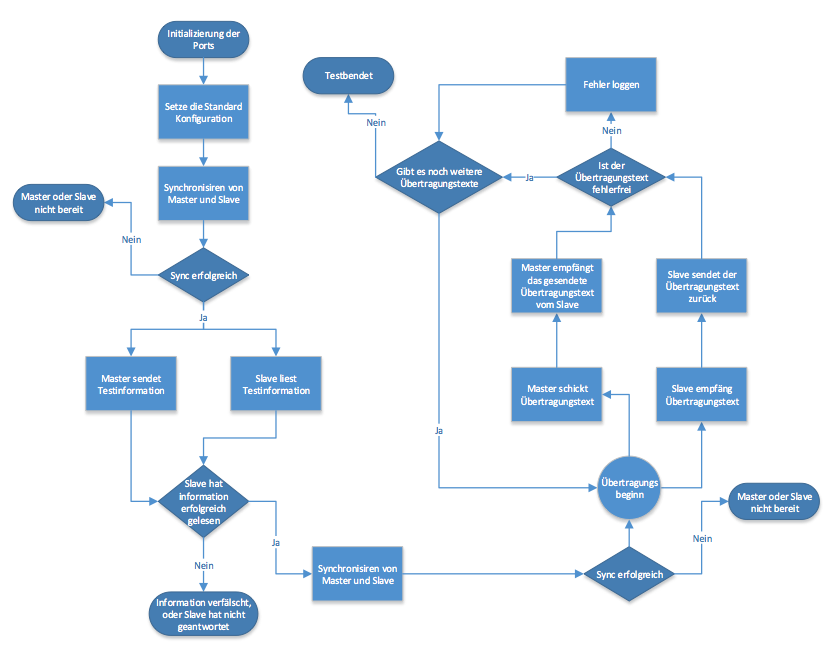
\includegraphics[scale=0.5]{MasterSlave.png}
  		  \caption{Ablauf des Master-Slave Test}
     \label{MasterSlaveDiagramm}
  \end{center}
\end{figure}


\newpage


Die Synchronisation der beiden COM Ports geschieht indem der Master ein Fluchtzeichen (Escape-Sequenzen) schickt und der Slave antwortet. Der Master schickt ein "`ESC"' (ASCII 0x1B) und wartet auf die Antwort vom Slave, was in Form von einem "`ACK"' (ASCII 0x06) gesendet wird. Wenn beide COM Ports synchron sind, schick der Master dem Slave eine "`Kopfzeile"'. In dieser Kopfzeile steht die Nummer der zu übertragenden Zeile, so wie die Anzahl der zu übertragenen Bytes, jeweils mit einer Breite von drei Zeichen gesendet. Die Kopfzeile hat folgendes Format:

\begin{center}
<Zeilennummer-Anzahl\_An\_Bytes>\\

<001-010>
\end{center}

Die Kopfzeile ist nötig, damit der Slave weiß, wie viele Zeichen im Übertragungstext, bei der nächsten Übertragung, ankommen werden, damit die richtige Anzahl an Bytes aus dem Puffer gelesen werden kann. Nachdem die Kopfzeile empfangen worden ist, und der Slave sein Inhalt interpretieren kann, wird ein "`ACK"' gesendet, damit der Master weiß, dass die Kopfzeile erfolgreich übertragen worden ist. Wenn der Master das "`ACK"' aus seinen Puffer liest, schickt er die erste Information an den Slave zurück. Diese Information ist die gewünschte Testeinstellung.

\begin{center}
baudrate;parität;stopbits;datenbits;protokoll\\
9600;1;2;8;2
\end{center}

Der Slave liest die ankommende Information und schickt ein "`ACK"' zurück. Danach wird die Information auf valide Werte überprüft und die Einstellungen werden gespeichert. In diesem Moment sind beide Schnittstellen synchron und bereit den Testvorgang mit den gewünschten Testeinstellungen zu starten. In beiden Schnittstellen werden die gewünschten Einstellungen gesetzt, und die Schnittstellen versuchen sich erneut zu synchronisieren. Ist die Synchronisation erfolgreich, schickt der Master erneut eine Kopfzeile an den Slave und danach der Übertragungstext. Der Slave antwortet auf die Kopfzeile beim erfolgreichen Empfangen mit einem "`ACK"' und beim Empfang vom Übertragungstext wird dieser zurück geschickt. Nachdem der Master den Übertragungstext versendet, wartet er auf die Antwort des Slaves in Form vom versendeten Text. Der Master liest den Empfangenen Text aus seinem Puffer und vergleicht es, mit dem versendeten Text. Werden keine Fehler festgestellt, wird der Vorgang wiederholt bis das Ende der Übertragung erreicht ist.


%****************************************************************************************
\newpage
%****************************************************************************************


\section{Klasse IniFileHandler}\label{IniFileHandler}
\paragraph{}
Die Klasse \textit{IniFileHandler} behandelt das Lesen und Speichern von Testeinstellungen in einer Datei, einer so genannten Testkonfigurationsdatei. Das Format dieser Datei basiert auf der von Windows vorgegebenen Initialisierungsdateien (.ini, INI-Datei). Mit Hilfe der Methoden \textit{WritePrivateProfileString}\footnote{http://msdn.microsoft.com/en-us/library/windows/desktop/ms725501(v=vs.85).aspx; 22.09.2013} und \textit{GetPrivateProfileString}\footnote{http://msdn.microsoft.com/en-us/library/windows/desktop/ms724353(v=vs.85).aspx; 22.09.2013} können jeweils die Testparameter geschrieben und gelesen werden. Das Format einer INI-Datei ist folgendermaßen aufgebaut:\\

\hspace*{20mm}\textit{[Sektion]}    \\
\hspace*{20mm}\textit{;Kommentar}    \\
\hspace*{20mm}\textit{Variable=Wert}\\

In Kapitel \ref{chp:bedienungsanleitung} werde genauer die Parameter und die Werte für einer Datei erläutert. Die Klasse ist in drei Arten von Methoden getrennt, diese sind Lese-, Schreib- und Übersetzermethoden.\\

\subsection{Übersetzer}
\paragraph{}
Die Übersetzermethoden bekommen einen Parameter, der entweder geschrieben oder im Programm gespeichert wird. In beiden Fällen muss der Parameter auf Gültigkeit geprüft werden. Wird der Parameter in einer INI-Datei geschrieben, muss er in manchen Fällen, wie zum Beispiel bei der Baudrate, zuerst von einer Zahl auf einen String umgewandelt werden. Wird die Baudrate gelesen, muss dieser String auf eine Zahl umgewandelt werden und geprüft werden, ob der gelesene/umgewandelte Wert ein gültiger Wert ist. Dieser Vorgang gilt für alle anderen Parametern auch.



\subsection{Schreiben}
\paragraph{}
Durch den Aufruf der Methode \textit{WritePrivateProfileString} mit folgenden Parameter wird die Baudrate in eine Datei gespeichert:\\

\begin{lstlisting}
WritePrivateProfileString(ComPort,"Baudrate","9600", Dateipfad);
\end{lstlisting}

Die Variable \textit{Dateipfad} spezifiziert die Zieldatei in der die Schlüssel/Variable \textit{Baudrate} geschrieben werden soll. Der Wert für den Eintrag ist \textit{9600}. Der Eingabeparameter \textit{ComPort} ist die Bezeichnung für einen COM Port und gibt an in welcher Sektion die Variable \textit{Baudrate} geschrieben werden soll. Der Eintrag für den Aufruf dieser Methode lautet:\\

\hspace*{20mm}\textit{[COM2]}    \\
\hspace*{20mm}\textit{;Das ist die Baudrate}    \\
\hspace*{20mm}\textit{Baudrate=9600}\\

Auf diese Weise werden alle Testeigenschaften in einer INI-Datei gespeichert. Durch die Trennung von Sektionen werden die Parameter für verschiedene COM Ports bei einem neuen Eintrag nicht überschrieben.


\subsection{Lesen}
\paragraph{}
Will der Benutzer Werte, beziehungsweise die Baudrate, aus einer INI-Datei lesen, muss er die Methode \textit{GetPrivateProfileString} mit folgenden Parametern aufrufen:\\

\begin{lstlisting}
GetPrivateProfileString(ComPort, "Baudrate", NULL,
                        Puffer, GrößeDesPuffers, Dateipfad);
\end{lstlisting}

Die bekannten Parameter sind die gleichen wie bei der Schreibmethode. \textit{Puffer} ist eine Variable, in der der gelesene Wert geschrieben wird und \textit{GrößeDesBuffers} gibt die Größe des Puffers an. So wird der String \textit{9600} in die Variable \textit{Puffer} geschrieben. Durch Aufruf der entsprechenden Übersetzermethode, wird die gelesene Baudrate in eine Zahl umgewandelt und im Programm gespeichert.


%****************************************************************************************
\newpage
%****************************************************************************************

\section{Klasse Tools}
\paragraph{}
Die Klasse \textit{Tools} ist eine Sammlung von verschiedenen Hilfsmethoden, die in den anderen Klassen aufgerufen werden.

  
\subsection{String Methoden}
\paragraph{}
In den anderen Klassen ist es immer wieder nötig Variablen in Strings umzuwandeln. Die Methode \textit{convertToString} konvertiert ganze Zahlen, Multibyte Zeichenketten und Zeiger auf Zeichenketten zu einem String. Der Eingabeparameter der Funktion wird in einen \textit{stringstream} geschrieben und dieser Stream wird als String zurückgegeben.\\

Eine weitere Methode heißt \textit{printTime}, diese Methode fragt die Uhrzeit im System ab und schreibt diese in einen String, der zurück gegeben wird. Die Methode \textit{delSpaces} löscht alle Leerzeichen in das an die Methode übergebene String. 

\begin{lstlisting}
	s.erase(remove_if(s.begin(), s.end(), isspace),s.end());
\end{lstlisting}

Der Löschvorgang wird mit Hilfe von der String-Klassenmethode \textit{erase} und der \textit{Template Class} \textit{remove\_if} durchgeführt. Die Anfang- und Enditeratoren des Strings werden an die \textit{Templa Class} gegeben somit wird das Zeichen markiert welches gelöscht werden soll. Die Zeichen sind alle Leerzeichenmöglichkeiten (Tabs, CarriageReturn, NewLine, etc.) zu verstehen, diese werden durch die Funktion \textit{isspace} abgefragt und von der \textit{erase} Methode gelöscht.\\

Die letzte Methode teilt die durch Leerzeichen übergebene Zeichenkette in einzelnen Strings und schreibt diese in einen Vektor vom Typ String. Diese Methode wird angewendet um die, über die Kommandozeile eingegebenen Parameter zu erkennen und einzeln auswerten zu können. Die letzte Stringmethode wird für den Übertragungstext benutzt. Wenn ein Übertragungstext so genannte Fluchtzeichen beinhalten soll, werden diese als Hexadezimalwerte eingegeben und in dieser Methode durch ein Zeichen ersetzt.

\subsection{Weitere Methoden}
\paragraph{}
Eine andere Art von Methoden in dieser Klasse ist die \textit{printErrorVector} Methode. Diese Methode gibt die Ergebnisse der Tests aus, jeweils über die GUI als Fenster oder in der Logdatei. Die Methode \textit{errorCodeParser} bekommt als Eingabeparameter ein Exitcode eines Funktionsaufrufes und gibt die Erklärung dieses Exitcodes als String zurück. Die \textit{wait} Methode bekommt eine Zahl als Eingabeparameter. Diese Zahl dient als Multiplikator mit dem die Zehn Millisekunden multipliziert werden, das Ergebnis ist die zu wartende Zeit. Die Methode wird bei der Synchronisierung von einen Master und einen Slave benutzt. Die letzte Methode in der Klasse \textit{Tools} zeigt dem Benutzer einen Hilfetext an, wenn falsche Eingabeparameter in der Kommandozeile eingegeben worden sind.



%****************************************************************************************
\newpage
%****************************************************************************************


\section{Klasse TransferFileHandler}
\paragraph{}
Die Klasse \textit{TransferFileHandler} behandelt die Dateien die in einer Übertragung gesendet werden sollen. Die Klasse öffnet, liest und schließt die Datei.

\subsection{Aufbau}
\paragraph{}
Die Klasse öffnet mittels der Methode \textit{openFile} eine Datei die als Eingabeparameter angegeben worden ist. Eine Variable vom Typ \textit{ifstream} (input file stream) wird deklariert. Durch die Methode \textit{open} wird der Pfad der Datei angegeben und die Methode versucht diese Datei zu öffnen. Falls die Datei nicht geöffnet werden konnte, wird der Benutzer benachrichtigt. Ist die Datei erfolgreich geöffnet worden, wird jede Zeile in der Datei bis zum Ende gelesen und in einem Vektor gespeichert. Danach wird die Datei geschlossen.\\


%****************************************************************************************
\section{Klasse Logger}\label{LoggerClass}
\paragraph{}
Die Klasse \textit{Logger} erzeugt auf Wunsch des Benutzers eine Logdatei, worin alle Testereignisse geschrieben werden. Wird ein Objekt von der Klasse \textit{Logger} erzeugt, wird als erstes eine Datei im "`\%temp\%"' Ordner angelegt und der Puffer des Objekts \textit{clog} (output stream) auf die Logdatei umgeleitet. Ein Beispiel einer Logdatei, bitte siehe Anhang ~\ref{LogDatei}.\\



%****************************************************************************************
\section{Header Constants}
\paragraph{}
In die Headerdatei \textit{Constants} werden alle Konstanten für das Programm deklariert. Unter anderem sind hier die Werte für:

\begin{itemize}
\item Programmversion
\item ID der GUI-Elemente
\item Errorcodes
\item Baudraten
\item TestStruct (siehe \ref{TestStruct})
\end{itemize}

deklariert.